%!TEX program = xelatex
\documentclass[11pt,a4paper]{article}
\usepackage[utf8]{inputenc}
\usepackage[T1]{fontenc}
\usepackage{authblk}
\usepackage{tikz}
\usepackage{pgfplots}
\usepackage{verbatim}
\usepackage{amsfonts}
\usepackage{amsmath}
\usepackage{amsthm}
\usepackage{indentfirst}
\usepackage{amssymb}
\usepackage{enumerate}
\linespread{1.6}
\setlength{\footskip}{20pt}
\setlength{\parindent}{0pt}
\usetikzlibrary{shapes,snakes}
\newcommand{\argmax}{\operatornamewithlimits{argmax}}
\newcommand{\argmin}{\operatornamewithlimits{argmin}}
\DeclareMathOperator{\col}{col}
\usepackage{booktabs}
\newtheorem{theorem}{Theorem}
\newtheorem{note}{Note}
\newtheorem{definition}{Definition}
\newtheorem{proposition}{Proposition}
\newtheorem{lemma}{Lemma}
\newtheorem{example}{Example}
\newtheorem{corollary}{Corollary}
\usepackage{graphicx}
\usepackage{geometry}
\usepackage{hyperref}
\newcommand{\code}{	exttt}
\geometry{a4paper,scale=0.8}
\title{Notes of Probability}
\author[*]{Wenxiao Yang}
\affil[*]{Department of Mathematics, University of Illinois at Urbana-Champaign}
\date{Last updated: 2022.09}


\begin{document}
\maketitle
\tableofcontents
\newpage

\section{Distribution}

\subsection{Discrete}
\subsubsection{Bernoulli Distribution -- $\operatorname{Bernoulli}(\pi)$: an event happens with probability $\pi$}
Assume $n$ independent binary (taking values $0$ or $1$) observations arising from independent and identical trials: $y_{1}, y_{2}, \ldots, y_{n}$ such that: $P\left(Y_{i}=1\right)=\pi$ and $P\left(Y_{i}=0\right)=1-\pi$.

Random variables $Y_{i}$ are normally called \textbf{Bernoulli} trials, $Y_{i} \sim \operatorname{Bernoulli}(\pi)$. $$\mathbb{E}(Y_i)=\pi,Var(Y_i)=\pi(1-\pi)$$

\subsubsection{Binomial distribution -- $bin(n,\pi)$: $n$ independent Bernoulli distributions}
The random variable $Y=\sum_{i=1}^{n} Y_{i}$ has the Binomial distribution with index $n$ and parameter $\pi$ denoted as $Y \sim \operatorname{bin}(n, \pi)$.
Mass probability function for $Y$ :
$$
P(y)=\left(\begin{array}{l}
n \\
y
\end{array}\right) \pi^{y}(1-\pi)^{n-y}
$$
with $\left(\begin{array}{l}n \\ y\end{array}\right)=\frac{n !}{y !(n-y) !}$ and $y=0,1,2, \ldots, n$
\begin{enumerate}[(1)]
    \item Mean and Variance:
    $\mathbb{E}(Y)=\mu=n \pi,\operatorname{Var}(Y)=\sigma^{2}=n \pi(1-\pi)$
    \item Skewness: $\mathbb{E}\frac{(Y-\mu)^{3}}{\sigma^{3}}=\frac{1-2 \pi}{\sqrt{n \pi(1-\pi)}}$
    \item If the independence assumption is violated, the Binomial distribution does not apply.
    \item Normal approximation:$\frac{Y-n \pi}{\sqrt{n \pi(1-\pi)}} \stackrel{d}{\longrightarrow} N(0,1),\quad {n \rightarrow \infty}$.
\end{enumerate}

\subsubsection{Multinomial Distribution}

\subsubsection{Poisson Distribution -- $Pois(\lambda)$: an event happens $k$ times within unit time}
$\lambda$: frequency of the event, i.e., the average number of event happens within unit time.
$$\Pr(X{=}k)= \frac{\lambda^k e^{-\lambda}}{k!},\ k=0,1,2,3...$$
$$E(X)=Var(X)=\lambda$$

\subsubsection*{Derivation process:}
Consider a unit time (the unit is divided into $n$ equal subparts, $n \rightarrow \infty$), there is an event may occur with every subpart, the number of the event happens should follow binomial distribution $B(n,p)$. where $n \rightarrow \infty, p \rightarrow 0$; $\lambda=n\cdot p$ is the expected number of events in this period of time.

the probability the number of the event happens:
\begin{equation}
    \begin{aligned}
        \Pr(X=k)&=\lim_{n \rightarrow\infty} \binom{n}{k} (\frac{\lambda}{n})^k(1-\frac{\lambda}{n})^{n-k}\\
        &=\lim_{n \rightarrow\infty} \frac{n!}{(n-k)!k!} (\frac{\lambda}{n})^k(1-\frac{\lambda}{n})^{n}(1-\frac{\lambda}{n})^{-k}\\
        &=\lim_{n \rightarrow\infty}\frac{n!}{(n-k)!k!} (\frac{\lambda}{n})^k e^{-\lambda}\\
        &=\frac{\lambda^k e^{-\lambda}}{k!}\lim_{n \rightarrow\infty}\frac{n!}{(n-k)!n^k}\\
        &=\frac{\lambda^k e^{-\lambda}}{k!}\lim_{n \rightarrow\infty}
        \frac{n}{n}\frac{n-1}{n}\cdots \frac{n-k+1}{n}\\
        &=\frac{\lambda^k e^{-\lambda}}{k!}
    \end{aligned}
    \nonumber
\end{equation}

\subsubsection*{Sums of independent Poisson random variables are Poisson random variables}
$X\sim Pois(\lambda_1), Y\sim Pois(\lambda_2)$ are two independent Poisson random variables, then $Z=X+Y$ also follow Poisson distribution, and the paramenter is the sum of $X$'s and $Y$'s
\begin{equation}
    \begin{aligned}
        Z\sim Pois(\lambda_1+\lambda_2)
    \end{aligned}
    \nonumber
\end{equation}
Then, $$Z=X_1+X_2+\cdots+X_n\sim Pois(\lambda_1+\lambda_2+\cdots+\lambda_n)$$

\subsection{Continuous}
\subsubsection{Exponential distribution $Exp(\lambda)$: interval between to independent identical event / the first time a event happened}
$\lambda$: frequency of the event.

$X$ follows exponential distribution with parameter $\lambda$ or $\beta$:
$${\displaystyle X\sim {\text{Exp}}(\lambda )} \text{ or } {\displaystyle X\sim {\text{Exp}}(\beta )}$$
They are equivlanet, the only difference is $\beta=\frac{1}{\lambda}$.
$${f(x;{\lambda})=\left\{{\begin{matrix}{\lambda }e^{-{\lambda }x}&x\geq 0\\0&\;x<0.\end{matrix}}\right.}$$
$${f(x;{\beta})=\left\{{\begin{matrix}{\frac{1}{\beta} }e^{-{\frac{1}{\beta} }x}&x\geq 0\\0&\;x<0.\end{matrix}}\right.}$$
c.d.f is:
$${F(x;{\lambda})=\left\{{\begin{matrix}{1-}e^{-{\lambda }x}&x\geq 0\\0&\;x<0.\end{matrix}}\right.}$$
Note that $\lambda > 0$ is the frequcy of the occurance of the event; $\beta>0$ is the probability of the event happens in each second. The range of exponential distribution is $[0,\infty)$.

$\mathbb{E}(X)=\frac{1}{\lambda}$; $Var(X)=\frac{1}{\lambda^2}$
$$\mathbb{E}(X)=\frac{1}{\lambda};\ Var(X)=\frac{1}{\lambda^2}$$
Memorylessness: ${\displaystyle \Pr \left(T>s+t\mid T>s\right)=\Pr(T>t)}$
\begin{equation}
    \begin{aligned}
        \Pr (T>s+t\mid T>s)&=\frac{\Pr(T>s+t\text{ and }T>s)}{\Pr(T>s)}\\
        &=\frac{\Pr(T>s+t)}{\Pr(T>s)}\\
        &=\frac{e^{-\lambda(s+t)}}{e^{-\lambda s}}\\
        &=e^{-\lambda t}\\
        &=\Pr (T>t)
    \end{aligned}
    \nonumber
\end{equation}

\subsubsection*{Derivation process:}

Consider a unit time (the unit is divided into $n$ equal subparts, $n \rightarrow \infty$), there is an event may occur with every subpart, the number of the event happens should follow binomial distribution $B(n,p)$. where $n \rightarrow \infty, p \rightarrow 0$; $\lambda=n\cdot p$ is the expected number of events in this period of time. (the same as Poisson)\\
CDF:
\begin{equation}
    \begin{aligned}
        1-F(x;\lambda)=\lim_{n \rightarrow \infty}(1-\frac{\lambda}{n})^{nx}=e^{-\lambda x}
        \Rightarrow F(x;\lambda)=1-e^{-\lambda x}
    \end{aligned}
    \nonumber
\end{equation}
PDF:
\begin{equation}
    \begin{aligned}
        f(x;\lambda)=\frac{\partial F(x;\lambda)}{\partial x}=\lambda e^{-\lambda x}
    \end{aligned}
    \nonumber
\end{equation}

\subsubsection{Gaussian/Normal Distribution}
$N(\mu,\sigma^2)$. p.d.f. ${\displaystyle f(x)={\frac {1}{\sigma {\sqrt {2\pi }}}}e^{-{\frac {1}{2}}\left({\frac {x-\mu }{\sigma }}\right)^{2}}}$
\begin{theorem}
Suppose $X\sim N(\mu_1,\sigma_1^2)$ and $Y\sim N(\mu_2,\sigma_2^2)$ are independent, then $X+Y\sim N(\mu_1+\mu_2,\sigma_1^2+\sigma^2)$.
\end{theorem}
\begin{proof}
The MGF of $X$ is
\begin{equation}
    \begin{aligned}
        M_X(t)=\mathbb{E}e^{tx}&=\int_{-\infty}^{\infty}e^{tx}\frac{1}{\sqrt{2\pi}\sigma_1}e^{-\frac{(x-\mu_1)^2}{2\sigma_1^2}}dx\\
        &=\int_{-\infty}^{\infty}\frac{1}{\sqrt{2\pi}\sigma_1}e^{-\frac{x^2-2(\mu_1+\sigma_1^2t)x+\mu_1^2}{2\sigma_1^2}}dx\\
        &=e^{\frac{\sigma_1^4t^2+2\mu_1\sigma^2t}{2\sigma_1^2}}\int_{-\infty}^{\infty}\frac{1}{\sqrt{2\pi}\sigma_1}e^{-\frac{(x-(\mu_1+\sigma_1^2t))^2}{2\sigma_1^2}}dx\\
        &=e^{t\mu_1+\frac{1}{2}\sigma_1^2t^2}
    \end{aligned}
    \nonumber
\end{equation}
Then, the MGF of $X+Y$ is
\begin{equation}
    \begin{aligned}
        M_{X+Y}(t)=\mathbb{E}e^{t(X+Y)}=\mathbb{E}e^{tX}\mathbb{E}e^{tY}=e^{t(\mu_1+\mu_2)+\frac{1}{2}(\sigma_1^2+\sigma_2^2)t^2}=M_{Z}(t)
    \end{aligned}
    \nonumber
\end{equation}
where $Z\sim N(\mu_1+\mu_2,\sigma_1^2+\sigma^2)$
\end{proof}

\subsubsection{Multivariate/Joint Gaussian/Normal Distribution (MVN)}
A $k$-dimensional random vector $(X_1,X_2,...,X_k)^T=\mathbf{X}\sim N(\mu,\Sigma)$.

p.d.f. $${\displaystyle f_{\mathbf {X} }(x_{1},\ldots ,x_{k})={\frac {\exp \left(-{\frac {1}{2}}({\mathbf {x} }-{\boldsymbol {\mu }})^{\mathrm {T} }{\boldsymbol {\Sigma }}^{-1}({\mathbf {x} }-{\boldsymbol {\mu }})\right)}{\sqrt {(2\pi )^{k}|{\boldsymbol {\Sigma }}|}}}}$$

A random vector is said to be $k$-variate normally distributed if every linear combination of its $k$ components has a univariate normal distribution.
\begin{enumerate}[(1)]
    \item $\mu$ is a $k$-dimensional \textbf{mean vector}: $$\mu=\mathbb{E}[\mathbf{X}]=(\mathbb{E}[X_1],\mathbb{E}[X_2],...,\mathbb{E}[X_k])^T$$
    \item $\Sigma$ is a $k\times k$ \textbf{covariance matrix}$${\displaystyle \Sigma _{i,j}=\operatorname {E} [(X_{i}-\mu _{i})(X_{j}-\mu _{j})]=\operatorname {Cov} [X_{i},X_{j}]}$$
    \item The inverse of $\Sigma$, ${\boldsymbol {Q}}={\Sigma }^{-1}$ is \textbf{precision matrix}.
\end{enumerate}
\begin{theorem}
    MVN distribution is completely specified by knowing $\mu$, $\Sigma$.
\end{theorem}
\begin{proof}
MGF: $M_X(t_1,t_2,...,t_k)=\mathbb{E}e^{\sum_{i=1}^k t_ix_i}$

Since any linear combination of $X$ is also normal distribution, $\Omega=\sum_{i=1}^k t_ix_i$ follows normal distribution.
$$M_X(t_1,t_2,...,t_k)=\mathbb{E}e^\Omega=e^{\mathbb{E}(\Omega)+\frac{1}{2}Var(\Omega)}=e^{\sum_{i=1}^kt_i \mathbb{E}(x_i)+\frac{1}{2}Var(\sum_{i=1}^k t_ix_i)}$$
\end{proof}

Generally, "independence" is a \textbf{stronger} condition than "$0$ correlation" ($Cov=0$).
\begin{theorem}
    For \textbf{MVN}, "independence" is \textbf{equivalent} to "$0$ correlation"
\end{theorem}
\begin{proof}
As we show $M_X(t_1,t_2,...,t_k)=e^{\sum_{i=1}^kt_i \mathbb{E}(x_i)+\frac{1}{2}Var(\sum_{i=1}^k t_ix_i)}$. If $Cov(x_i,x_j)=0,\forall i,j\in S$,
\begin{equation}
    \begin{aligned}
        M_X(t_1,t_2,...,t_k)&=e^{\sum_{i=1}^kt_i \mathbb{E}(x_i)+\frac{1}{2}Var(\sum_{i=1}^k t_ix_i)}\\
        &=e^{\sum_{i=1}^it_ki \mathbb{E}(x_i)+\frac{1}{2}\sum_{i=1}^it_i^2Var(x_i)}\\
        &=\prod_{i=1}^ke^{t_i\mathbb{E}(x_i)+\frac{1}{2}t_i^2Var(x_i)}\\
        &=\prod_{i=1}^kM_{x_i}(t_i)
    \end{aligned}
    \nonumber
\end{equation}
\end{proof}

\begin{theorem}
    Independent $X=[X_1,X_2,...,X_n]\sim$ MVN and $Y=[Y_1,Y_2,...,Y_m]\sim$ MVN, then $W=[X_1,X_2,...,X_n,Y_1,Y_2,...,Y_m]\sim$ MVN.
\end{theorem}

\begin{theorem}
    Independent $X=[X_1,X_2,...,X_n]\sim N(\mu_1,\Sigma_1)$ and $Y=[Y_1,Y_2,...,Y_n]\sim N(\mu_2,\Sigma_2)$, then $X+Y\sim N(\mu_1+\mu_2,\Sigma_1+\Sigma_2)$.
\end{theorem}














\subsection{Poisson process: A sequence of arrivals in continuous time with rate $\lambda$}
\subsubsection{Definition}
$N(t)\sim Pois(\lambda t)$: Number of arrivals in length $t$ follows Poisson distribution
\begin{equation}
    \begin{aligned}
        N(t)\sim Pois(\lambda t)\\
        \Pr(N(t)=k)=\frac{(\lambda t)^k e^{-\lambda t}}{k!}
    \end{aligned}
    \nonumber
\end{equation}
The number of arrivals in disjoint time intervals are independent.
\subsubsection{$T_j$: time of $j^{th}$ arrival}
$T_1>t$ is same as $N(t)=0$: $P(T_1>t)=P(N(t)=0)=e^{-\lambda t}$\\
$\Rightarrow T_1\sim Expo(\lambda) \Rightarrow T_j-T_{j-1}\sim Expo(\lambda); T_j\sim Gamma(j,\lambda)$

\subsubsection{Theorem (Conditional counts): $N(t_1)|N(t_2)=n\sim Bin(n,\frac{t_1}{t_2})$}
(We can interpret the theorem as: $n$ points distribute uniformly in $(0,t_2]$, so the probability a point loctae within $(0,t_1]$ is $\frac{t_1}{t_2}$)

\section{Basis}
\subsection{Covariance and Variance}
\begin{enumerate}[(1)]
    \item $\sigma_{XY}=Cov(X,Y)=\mathbb{E}\left[(X-\mathbb{E}X)(Y-\mathbb{E}Y)\right]=\mathbb{E}(XY)-\mathbb{E}X\mathbb{E}Y$
    \item $Cov(aX+b,Y)=aCov(X,Y)$
    \item $Cov(X+Y,W)=Cov(X,W)+Cov(Y,W)$
    \item $Cov(aX+bY,cX+dY)=ac\ {Var}(X)+(ad+bc)Cov(X,Y)+bd\ {Var}(Y)$
    \item $Var(aX+bY)=a^2\ {Var}(X)+2ab\ Cov(X,Y)+b^2\ {Var}(Y)$
\end{enumerate}
\subsection{Conditional Expectation and Variance}
\begin{enumerate}[(1)]
    \item Conditional variance: $$Var(Y|X=x)=\mathbb{E}\left((Y-\mathbb{E}(Y|X=x))^2|X=x\right)
    =\mathbb{E}(Y^2|X=x)-(\mathbb{E}(Y|X=x))^2$$
    \item \textbf{Law of Total Expectation:} $$\mathbb{E}(Y)=\sum_{i=1}^n \mathbb{E}(Y|A_i)P(A_i)$$
    \item \textbf{Law of Iterated Expectation (Adam's Law):}
    $$\mathbb{E}\left[\mathbb{E}(Y|X)\right]=\mathbb{E}(Y)$$
    \item \textbf{Adam's Law with extra conditioning:} $$\mathbb{E}\left(\mathbb{E}(Y|X,Z)|Z\right)=\mathbb{E}(Y|Z)$$
    \item \textbf{Law of Total Variance:}$$Var(Y)=\mathbb{E}(Var(Y|X))+Var(\mathbb{E}(Y|X))$$
\end{enumerate}

\subsection{Gambler's Ruin}
Suppose a gambler at each round either wins a dollar or loses a dollar with probability $\frac{1}{2}$ each. Suppose the gambler starts at $k$ dollars. He stops when either he reaches his goal of $N$ dollars or he goes bankrupt and loses all his money.

Let $A$ be the event that the gambler is ruined.
\begin{equation}
    \begin{aligned}
        P(A|x=k)=\frac{1}{2}P(A|x=k-1)+\frac{1}{2}P(A|x=k+1)\\
        \Rightarrow p_k-p_{k-1}=p_{k+1}-p_k
    \end{aligned}
    \nonumber
\end{equation}
According to the setting, $p_0=1,p_N=0$, then $p_k=\frac{N-k}{N}$.

\subsection{Moment Generating Function (MGF)}
Let $X$ be a random variable. The moment generating function (mgf) of $X$, denoted by $M_X(t)$:
\begin{equation}
    \begin{aligned}
        \underline{M_X(t)=\mathbb{E}[e^{tX}]}=\mathbb{E}\left[1+tX+\frac{(tX)^2}{2!}+\frac{(tX)^3}{3!}+\cdots\right]=\sum_{n=0}^\infty\frac{\mathbb{E}[X^n]t^n}{n!}
    \end{aligned}
    \nonumber
\end{equation}
We can find $\frac{\partial M_X(t)}{\partial t}= \mathbb{E}\left[Xe^{tX}\right]$, then $\frac{\partial M_X(0)}{\partial t}= \mathbb{E}\left[X\right]$. More generally, we can find that $$\frac{\partial^n M_X(0)}{\partial t^n}= \mathbb{E}\left[X^n\right],n=1,2,...$$
\subsubsection*{Why MGF is useful?}
\begin{enumerate}[(1)]
    \item If $X,Y$ are independent, then $$M_{X+Y}(t)=\mathbb{E}[e^{(X+Y)t}]=\mathbb{E}[e^tX]\mathbb{E}[e^tY]=M_X(t)M_Y(t)$$
    \item Unique random variable (RV) $\Leftrightarrow$ unique MGF
\end{enumerate}

\subsection{Inequality}
\subsubsection{Cauchy-Schwarz inequality: $|\mathbb{E}XY|\leq \sqrt{\mathbb{E}X^2\cdot \mathbb{E}Y^2}$}
For any r.vs. $X$ and $Y$ with finite variance: $|\mathbb{E}XY|\leq \sqrt{\mathbb{E}X^2\cdot \mathbb{E}Y^2}$
\begin{example}[Second Moment Method]
$X$ is a non-negative r.v. We want to find an \underline{upper bound} on $P(X=0)$.
\end{example}
Because $X$ is non-negative, $X=X\cdot \textbf{I}_{X>0}=\left\{\begin{matrix}
    X,&X>0\\
    0,&X=0
\end{matrix}\right.$. Hence,
\begin{equation}
    \begin{aligned}
        \mathbb{E}X= \mathbb{E}X\cdot \textbf{I}_{X>0}\leq \sqrt{\mathbb{E} X^2\cdot \textbf{I}^2_{X>0}}=\sqrt{\mathbb{E}X^2}\sqrt{P(X>0)}\\
        \Rightarrow P(X>0)\geq\frac{(\mathbb{E}X)^2}{\mathbb{E}X^2} \Rightarrow P(X=0)=1-P(X>0)\leq \frac{Var(X)}{\mathbb{E}X^2}
    \end{aligned}
    \nonumber
\end{equation}

\subsubsection{Jensen's Inequality: convex $g$ $\Rightarrow$ $\mathbb{E}(g(X))\geq g(\mathbb{E}(X))$}
If $g$ is convex $\mathbb{E}(g(X))\geq g(\mathbb{E}X)$; If $g$ is concave $\mathbb{E}(g(X))\leq g(\mathbb{E}X)$.

\subsubsection{Markov's Inequality: $P(|X|\geq a)\leq \frac{\mathbb{E}|X|}{a}$}
For any r.v. $X$ and a constant $a>0$. $P(|X|\geq a)\leq \frac{\mathbb{E}|X|}{a}$
\begin{proof}
$Y=\frac{|X|}{a}$, $Y\geq \mathbb{I}_{Y\geq 1} \Rightarrow \mathbb{E}Y\geq P(Y\geq 1) \Rightarrow \frac{\mathbb{E}|X|}{a}\geq P(|X|\geq a)$
\end{proof}
\textbf{Note:} Markov's Inequality can also be written as $P(X\geq a)\leq \frac{\mathbb{E}X}{a}$, $a>0$, $X$ is non-negative r.v.

\subsubsection{Chebychev's inequality: $P(|X-\mu|\geq a)\leq \frac{\sigma^2}{a^2}$}
Let $X$ be any r.v. with mean $\mu$, variance $\sigma^2<\infty$. Then for $a>0$, $P(|X-\mu|\geq a)\leq \frac{\sigma^2}{a^2}$.
\begin{proof}
$P(|X-\mu|\geq a)=P((X
-\mu)^2\geq a^2)\leq \frac{\mathbb{E}(X-\mu)^2}{a^2}=\frac{\sigma^2}{a^2}$
\end{proof}

\subsubsection{Chernoff Inequality: $P(X\geq a)\leq \frac{\mathbb{E}e^{tX}}{e^{ta}}$}
For any r.v. $X$ and constant $a>0,t>0$. $P(X\geq a)\leq \frac{\mathbb{E}e^{tX}}{e^{ta}}$
\begin{proof}
$P(X\geq a)=P(e^{tX}\geq e^{ta})\leq \frac{\mathbb{E}e^{tX}}{e^{ta}}$
\end{proof}

\subsection{Law of Large Numbers (LLN)}
Describe the behavior of the sample mean of i.i.d. as the sample size grows.

$x_{1}, x_{2}, \ldots, x_{n}$ i.i.d. with some distribution. $\mu<\infty,\sigma^{2}<\infty$,$\bar{x}=\frac{1}{n}\left(x_{1}+x_{2}+\cdots+x_{n}\right)$.
\subsubsection{Weak Law of Large Numbers (wLLN)}
\begin{theorem}[Weak Law of Large Numbers (wLLN)]
    The weak law of large numbers (also called Khinchin's law) states that the sample average \underline{converges in probability} towards the expected value.
    $${\displaystyle {\begin{matrix}{}\\{\overline {X}}_{n}\ {\xrightarrow {P}}\ \mu \qquad {\text{when}}\ n\to \infty .\\{}\end{matrix}}}$$
    That is, for any positive number $\varepsilon$,
    $${\displaystyle \lim _{n\to \infty }\Pr \!\left(\,|{\overline {X}}_{n}-\mu |<\varepsilon \,\right)=1.}$$
\end{theorem}
\begin{proof}
Prove by Chebychev's inequality.
$$
\begin{aligned}
&P(|\bar{x}-\mu|\geq\varepsilon) \leq \frac{\sigma^{2}}{n \varepsilon^{2}} \quad (Var\bar{x}=\frac{\sigma^{2}}{n}) \\
&\lim_{n \rightarrow \infty}\frac{\sigma^{2}}{n \varepsilon^{2}}=0\\
\Rightarrow&\lim_{n \rightarrow \infty}P(|\bar{x}-\mu|>\varepsilon) \text { also converges to } 0 .
\end{aligned}
$$
\end{proof}

\subsubsection{Strong Law of Large Numbers (sLLN)}
\begin{theorem}[Strong Law of Large Numbers (sLLN)]
    \quad

    With probability 1 (wp1) or almost surely (as).
    $${\displaystyle {\begin{matrix}{}\\{\overline {X}}_{n}\ {\xrightarrow {a.s.}}\ \mu \qquad {\text{when}}\ n\to \infty .\\{}\end{matrix}}}$$

    That is,
    $$\Pr \!\left(\lim _{n\to \infty }{\overline {X}}_{n}=\mu \right)=1.$$
\end{theorem}

\subsubsection{Differences between \underline{convergence in probability} (wLLN) and \underline{wp1(a.s.)} (sLLN)}
\begin{enumerate}[a)]
    \item Weak Law of Large Numbers (wLLN)
    $$P(|\bar{x}-\mu|\geq\varepsilon)\rightarrow 0\text{ as }n \rightarrow	+\infty,\ \forall \varepsilon>0$$
    \begin{center}\begin{figure}[htbp]
        \centering
        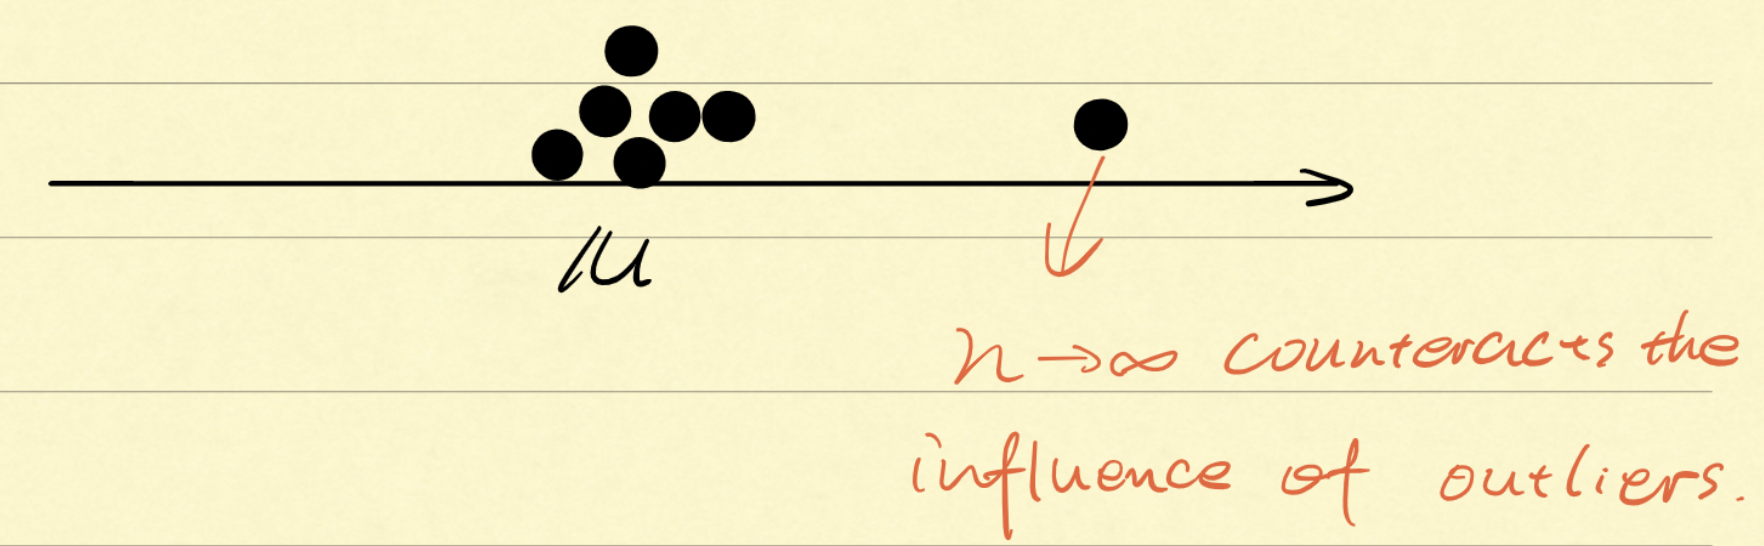
\includegraphics[scale=0.3]{wLLN.png}
        \caption{convergence in probability}
        \label{}
    \end{figure}\end{center}
    \item Strong Law of Large Numbers (sLLN)
    $$P(|\bar{x}-\mu|\geq\varepsilon\text{ as }n \rightarrow+\infty)=0,\ \forall \varepsilon>0$$
    \begin{center}\begin{figure}[htbp]
        \centering
        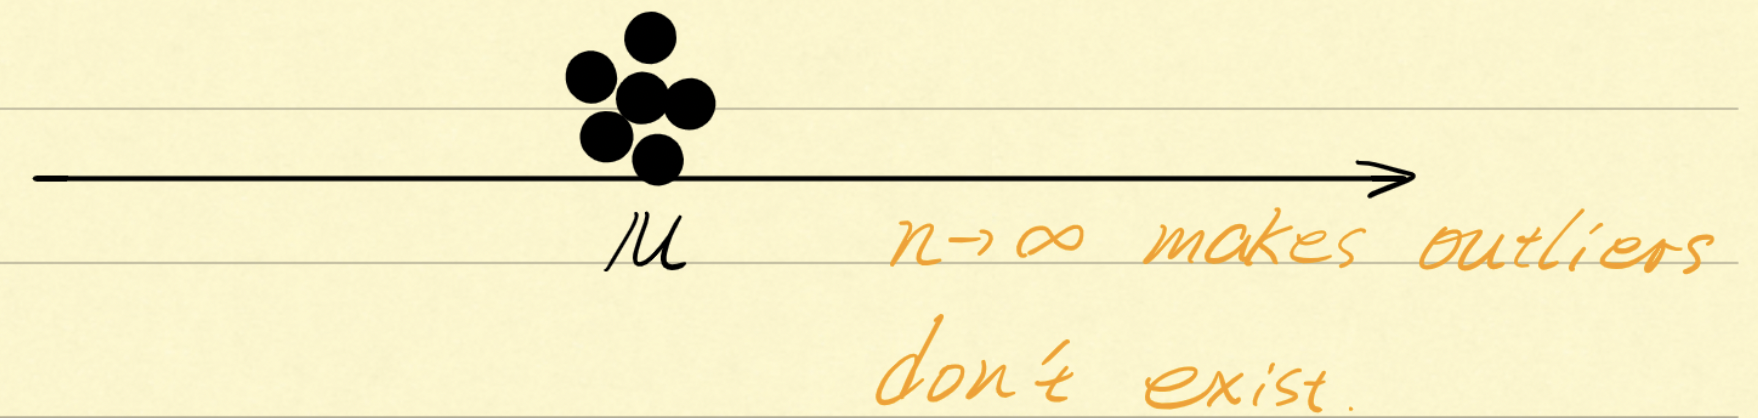
\includegraphics[scale=0.3]{sLLN.png}
        \caption{wp1(a.s.)}
        \label{}
    \end{figure}\end{center}
\end{enumerate}

\subsection{Central Limit Theorem (CLT)}
\begin{theorem}[Central Limit Theorem (CLT)]
    $$Z=\frac{\overline{X}-\mu}{\frac{\sigma}{\sqrt{n}}} \xrightarrow {D} N(0,1) \text{ when}\ n\to \infty$$
    $Z$ \underline{converges in distribution} to $N(0,1)$ as $n\to \infty$

    (converges in distribution: $P(\frac{\overline{X}-\mu}{\frac{\sigma}{\sqrt{n}}}\leq a)\rightarrow \frac{1}{\sqrt{2\pi}}\int_{-\infty}^ae^{-\frac{x^2}{2}}dx$)
\end{theorem}
\begin{proof}
    Prove the situation of $\mu=0,\sigma^2=1$, we can use linear transformations to get other situations.

    Moment-generating function(MGF) of $X_i$: $M_0(t)=E(e^{tX_i})$. $$M_0(0)=1,M_0'(0)=EX_i=0,M_0''(0)=EX_i^2=1$$
    Moment-generating function(MGF) of $\sqrt{n}\overline{X}$:
    \begin{equation}
        \begin{aligned}
            M_1(t)&=Ee^{t\sqrt{n}\overline{X}}=Ee^{t\frac{\sum_{i=1}^nX_i}{\sqrt{n}}}\\
            &=Ee^{t\frac{X_1}{\sqrt{n}}}\cdot Ee^{t\frac{X_2}{\sqrt{n}}}\cdots Ee^{t\frac{X_n}{\sqrt{n}}}\\
            &=[M_0(\frac{t}{\sqrt{n}})]^n
        \end{aligned}
        \nonumber
    \end{equation}
    \begin{equation}
        \begin{aligned}
            \lim_{n \rightarrow	\infty}\log M_1(t)&=\lim_{n \rightarrow	\infty}n\log M_0(\frac{t}{\sqrt{n}})\\
            &(\text{let }y=\frac{1}{\sqrt{n}})\\
            &=\lim_{y=0}\frac{\log M_0(yt)}{y^2}\\
            &(\text{L'Hôpital's rule})\\
            &=\lim_{y=0}\frac{t M'_0(yt)}{2y M_0(yt)}\\
            &(\text{L'Hôpital's rule})\\
            &=\lim_{y=0}\frac{t^2 M''_0(yt)}{2 M_0(yt)+2ytM'(yt)}\\
            &=\frac{t^2}{2}
        \end{aligned}
        \nonumber
    \end{equation}
    As we know the Moment-generating function(MGF) of $Z\sim N(0,1)$ is $M_Z(t)=\frac{t^2}{2}$.

    Hence, $M_1(t)=M_Z(t)$ i.e. $\frac{\overline{X}-\mu}{\frac{\sigma}{\sqrt{n}}} \xrightarrow {D} N(0,1)$ as $n \rightarrow\infty$
\end{proof}



\section{Markov Chain}
\subsection{Definition}
For discrete state space $S$, a Markov Chain is a stochastic process $X_0,X_1,X_2,...$   such that$$P(X_{n+1}=i|X_n=j,X_{n-1}=x_{n-1},...,X_0=x_0)=P(X_{n+1}=i|X_n=j)$$
for all $n\in \mathbb{Z}$ and $x_0,x_1,...,x_{n-1},i,j\in S$.

A MC is called \underline{time homogeneous} if $P(X_{n+1}=i|X_n=j)=P(X_1|X_0=j),\forall n\in \mathbb{Z}^+$ and $i,j\in S$ (we only consider time homogeneous MC).

The \textbf{transition probabilities} for a \underline{time homogeneous MC} can be written down as a matrix $P$ satisfying $P_{ij} = P (X_1 = j|X_0 = i)$. This matrix $P$ satisfies two properties:
\begin{enumerate}[(1)]
    \item $P_{ij}\geq 0$ for all $i,j\in S$.
    \item $\sum_{j\in S}P_{ij}=1$ for all $i\in S$.
\end{enumerate}
Any matrix satisfies the two properties is called a \textbf{stochastic matrix}.

\subsection{Matrix Computations}
Given a time homogeneous MC with initial distribution $X_0\sim\alpha\in [0,1]^{|S|}$ and transition matrix $P$.
\begin{lemma}[Distribution of Entire Sequence]
$$P(X_0=x_0,X_1=x_1,...,X_n=x_n)=P(X_0=x_0)P_{x_0,x_1}P_{x_1,x_2}...P_{x_{n-1},x_n}$$
\end{lemma}

\begin{lemma}[Markov Property]
    $$P(X_{t_n}=x_{t_n} | X_{t_{n-1}}=x_{t_{n-1}},...,X_{t_0}=x_{t_0})=P(X_{t_n}=x_{t_n}|X_{t_{n-1}}=x_{t_{n-1}})$$
\end{lemma}

\begin{lemma}[Transition Probability after $n$ states]
$$P(X_n=j|X_0=i)=(P^n)_{ij}$$
\end{lemma}
\begin{proof}
    $P(X_2=j|X_0=i)=\sum_{k\in S}P(X_2=j|X_1=k)P(X_1=k|X_0=i)=\sum_{k\in S}P_{kj}P_{ik}=(P^2)_{ij}$. Then prove by mathematical induction,
    $P(X_n=j|X_0=i)=\sum_{k\in S}P(X_n=j|X_{n-1}=k)P(X_{n-1}=k|X_0=i)=\cdots =(P^n)_{ij}$
\end{proof}

\subsubsection{Chapman Kolmogorov Equations (C-K Equations) $P(X_{n+m}=j|X_0=i)=(P^{m+n})_{ij}=\sum_{k\in S}(P^{m})_{ik}(P^{n})_{kj}$}
$m-$step transition probabilities from state $k$ to state $j$:
\begin{equation}
    P(X_{n+m}=j|X_0=i)=(P^{m+n})_{ij}=\sum_{k\in S}(P^{m})_{ik}(P^{n})_{kj}
\end{equation}
\begin{proof}
    $P(X_n=j|X_0=i)=\sum_{k\in S}P(X_{n+m}=j|X_{m}=k)P(X_{m}=k|X_0=i)=\sum_{k\in S}P(X_n=j|X_{0}=k)P(X_{m}=k|X_0=i)$
\end{proof}

\subsubsection{Marginal Distribution $P(X_n=j)=(\alpha P^n)_{j}$}
\begin{lemma}[Marginal Distribution]
    Given initial distribution $X_0\sim\alpha$ and transition matrix $P$. $\alpha$ is distribution vector ($1\times|S|$) with $\sum_{i\in S}{\alpha_i}=1$.
    $$P(X_n=j)=(\alpha P^n)_{j}$$
\end{lemma}
\begin{corollary}[Distribution of Subsequence]
    $$P(X_{t_{n}}=x_{t_{n}},X_{t_{n-1}}=x_{t_{n-1}},...,X_{t_0}=x_{t_0})=(\alpha P^{t_0})_{x_{t_0}}P^{t_1-t_0}_{x_{t_0},x_{t_1}}P^{t_2-t_1}_{x_{t_1},x_{t_2}}\cdots P^{t_{n}-t_{n-1}}_{x_{t_{n-1}},x_{t_{n}}}$$
\end{corollary}

\subsection{States, Class}
\subsubsection{Irreducible, Reducible}
\begin{enumerate}[$\bullet$]
    \item \underline{Accessible}: $j$ is accessible from $i$ if $\exists n$ s.t. $P_{ij}^n>0$.
    \item \underline{Communicate/Communication}: $i$ communicates $j$ ($i \leftrightarrow j$) if $j$ is accessible from $i$ and $i$ is accessible from $j$. (Reflexivity: $i \leftrightarrow i$; Symmetry: $i \leftrightarrow j$ $\Rightarrow$ $j \leftrightarrow i$; Transitivity: $i \leftrightarrow j$ and $j \leftrightarrow k$ $\Rightarrow$ $i \leftrightarrow k$.)
    \item \underline{(Communication) Class}: if $i \leftrightarrow j$, then states $i,j$ are said to be in the same \underline{(communication) class}. (Since communication is an equivalence relation, the state space can be partitioned into equivalence classes, called \textit{communication classes}.)
    \item \underline{Irreducible}: A Markov Chain that has \underline{only one class} is said to be \underline{irreducible}.
\end{enumerate}

\subsubsection{Recurrent, Transient}
\begin{enumerate}[$\bullet$]
    \item \underline{Recurrent State}: State $i$ is recurrent if $f_i=P($ever re-enter state $i$ if started in state $i)=1$. (the expected number of times it visits state $i$ is $\sum_{n=0}^\infty P_{ii}^n=+\infty$). (A MC is irreducible if all states are recurrent)
    \item \underline{Transient State}: State $i$ is transient if $f_i=P($ever re-enter state $i$ if started in state $i)<1$. (the expected number of times it visits state $i$ is $\sum_{n=0}^\infty P_{ii}^n<+\infty$; $P($visits state $i$ exactly $n$ times$)=f_i^{n-1}(1-f_i)$; The expected number is $\sum_{n=0}^\infty f_i^n(1-f_i)n={n=0}^\infty P_{ii}^n<\infty$).
    \item \underline{Transient Class}: A communicating class is called transient if starting from that class, with probability $1$ the MC leaves that class and never returns. The states of such a class are called transient states.
    \item \underline{Recurrent Class}: communicating class that is not transient.
    \begin{lemma}
        If $i$ is recurrent, $i\leftrightarrow j \Rightarrow$ $j$ is recurrent.
    \end{lemma}
    \begin{theorem}
        The states of a communication class are \underline{either all recurrent or all transient}.
    \end{theorem}
    \begin{corollary}
        For a \underline{finite irreducible} Markov chain, all states are recurrent.
    \end{corollary}
\end{enumerate}

\subsubsection*{Canonical Decomposition}
\begin{definition}
    A set of states $C$ is said to be \underline{closed} if no state outside of $C$ is accessible from any state in $C$. If $C$ is closed, then $$P_{ij} = 0,\ \forall i\in C,j\notin C$$
\end{definition}

\begin{lemma}
    (1) A communication class is \underline{closed} if it consists of all recurrent states.
    (2) A finite communication class is closed only if it consist of all recurrent states.
\end{lemma}
\begin{proof}
(1): if not closed, $\exists i\in C,j\notin C, P_{ij}>0$. $i$ shouldn't be accessible from $j$ since $i,j$ are not in one class. There exists positive probability that starting from $i$ then hit $j$ and never hit $i$ again, which contradicts to $i$ is recurrent. (2):According to former corollary, a finite class's all states are recurrent.
\end{proof}

\subsection{Periodicity}
Suppose $P$ is the transition matrix for an irreducible MC. For a given state $i$, we define the set $$J_i=\{n\geq 1:P^n(i,i)>0\}$$
$J_i$ is the set of times when it is possible for the MC to come back to $i$ starting from $i$ at time $0$. We define the \textbf{period} of a state $i$ is $$d(i)=gcd(J_i)$$
\subsubsection{Lemma: all states in an irreducible MC have the same period}
\begin{lemma}
    For an irreducible MC, all states have the same period.
\end{lemma}
\begin{proof}
    Let $d$ be a common divisor of $J_i$. Consider any other state $j$. We want to show $d$ is also the common divisor of $J_j$.
    
    Since the MC is irreducible, there exists $m$ and $n$ s.t. $P_{ij}^m>0$ and $P_{ji}^n>0$. Then $P_{ii}^{m+n}\geq P_{ij}^mP_{ji}^n >0 \Rightarrow m+n\in J_i$. $d$ should be a divisor of $m+n$.

    For any $l\in J_j$, $P_{ii}^{m+n+l}\geq P_{ij}^mP_{jj}^lP_{ji}^n >0 \Rightarrow m+n+l\in J_i$. $d$ divides $m+n+l$ $\Rightarrow$ $d$ divides $l$. Since $l$ can be any number in $J_j$, $d$ is a common divisor of $J_j$.
\end{proof}

\subsubsection{Periodic, Aperiodic}
A \underline{state} is \textbf{aperiodic} if period equals $1$, \textbf{periodic} otherwise.\\
A \underline{chain} is \textbf{aperiodic} if \underline{all} its states are aperiodic, \textbf{periodic} otherwise.

\subsection{Regular Matrix}
\subsubsection{Regular matrix: $\exists n\geq 1$ s.t. $P^n>0$}
A matrix $M$ is said to be positive if all the entries of $M$ are positive. We write $M > 0$.
\begin{definition}[Regular Transition Matrix]
    A transition matrix $P$ is said to be \underline{regular} if some power of $P$ is positive. That is, $P^n >0$, for some $n\geq 1$.
\end{definition}

\subsubsection{Lemma: Finite MC is Irreducible, Aperiodic $\Leftrightarrow$ has Regular transition matrix}
\begin{lemma}
    A finite MC is \textbf{irreducible} and \textbf{aperiodic} is equivalent to the transition matrix $P$ is \textbf{regular}.
\end{lemma}

We also call an MC is \textbf{ergodic} if it is \textbf{irreducible} and \textbf{aperiodic}.

\subsection{Long Run Behavior of Finite Markov Chains}
As $n \rightarrow \infty$, $P^n$:
\begin{enumerate}[(1)]
    \item Convergence. ($P^{n+1}=P^n$)
    \item Forgetting the initial states. (each row is identical)
\end{enumerate}


\subsubsection{Limiting Distribution}
\begin{definition}
    A MC is said to have a \textbf{limiting distribution} $\lambda$ if we have $$\lim_{n \rightarrow \infty}P_{ij}^n=\lambda_j,\ \forall i,j\in S$$
    An \underline{equivalent definition} is that for all initial distributions $X_0\sim \alpha$ and all $j\in S$ we have
    $$\lim_{n \rightarrow \infty}(\alpha P^n)_j=\lambda_j$$
\end{definition}

\textbf{Example: }$P=\begin{bmatrix}
    1-p&p\\
    q&1-q
\end{bmatrix}$. If $p+q=1$, each rows of $P$ is the same and $P^n=P$.

Assume $p+q\neq 1$,
\begin{equation}
    \begin{aligned}
        P^n_{11}&=P^{n-1}_{11}(1-p)+P^{n-1}_{12}q\\&=P^{n-1}_{11}(1-p)+(1-P^{n-1}_{11})q\\
        P^n_{11}&=\frac{q}{p+q}+\frac{p}{p+q}(1-p-q)^n \rightarrow \frac{q}{p+q}\text{ as }n \rightarrow \infty\\
        \lim_{n \rightarrow \infty}P^n&=\frac{1}{p+q}\begin{bmatrix}
            q&p\\
            q&p
        \end{bmatrix}
    \end{aligned}
    \nonumber
\end{equation}

\begin{lemma}
    If $\lambda$ is the limiting distribution for a MC with transition matrix $P$ then $\lambda$ satisfies the equation $$\lambda P=\lambda$$
\end{lemma}
\begin{proof}
    $(\lambda P)_j=\sum_{i\in S}\lambda_i P_{ij}=\sum_{i\in S}\lim_{n \rightarrow \infty}P_{ki}^nP_{ij}=\lim_{n \rightarrow \infty}\sum_{i\in S}P_{ki}^nP_{ij}=\lim_{n \rightarrow \infty}P_{kj}^{n+1}=\lambda_j$
\end{proof}

\subsubsection{Stationary Distribution}
\begin{definition}
    A distribution $\pi$ which satisfies the equation $$\pi P=\pi$$ is called a \textbf{stationary distribution} for the MC.
\end{definition}
\textbf{Note: }A limiting distribution $\lambda$ for the MC has to also be a stationary distribution. The converse is not always true.



\subsubsection{Limiting Distribution = Expected Proportion of time in each state}
The entries of the limiting distribution can also be interpreted as \textbf{the limit of the expected proportion of time the MC spends in each of the corresponding states.} For any state $j$, define the indicator random variable $I_k=1(X_k=j)$. Now define $$F_{n,j}=\frac{1}{n}\sum_{k=0}^{n-1}I_k$$
The random variable $F_{n,j}$ represents the proportion of time till time $n-1$ the MC spends in state $j$.

\begin{lemma}
    If $\lambda$ is the limiting distribution for a MC with transition matrix $P$ then $\lambda$ satisfies the equation $\lim_{n \rightarrow \infty}\mathbb{E}(F_{n,j}|X_0=i)=\lambda_j$ for all $j,i\in S$
\end{lemma}
\begin{proof}
    We can write $$\mathbb{E}(F_{n,j}|X_0=i)=\mathbb{E}\frac{1}{n}\sum_{k=0}^{n-1}\mathbb{E}(I_k|X_0=i)=\frac{1}{n}\sum_{k=0}^{n-1}P(X_k=j|X_0=i)=\frac{1}{n}\sum_{k=0}^{n-1}P_{ij}^k$$
    Therefore, taking limits we can conclude that $$\lim_{n \rightarrow \infty}\mathbb{E}(F_{n,j}|X_0=i)=\lim_{n \rightarrow \infty}\frac{1}{n}\sum_{k=0}^{n-1}P_{ij}^k=\lim_{n \rightarrow \infty}P_{ij}^n=\lambda_j$$
\end{proof}

\subsubsection{Fundamental Theorem for \underline{Irreducible, Aperiodic, Finite MC} (Regular transition matrix) $\Rightarrow $ $\exists$ unique limiting distribution $\pi$ and $\pi_j>0,\forall j$}
\begin{theorem}
    If $P$ is the transition matrix for an irreducible, aperiodic (finite) Markov chain then there exists a unique stationary distribution or a unique solution to the equation $\pi=\pi P$ which satisfies the following two properties:
    \begin{enumerate}[(1)]
        \item $\pi$ is the \textbf{limiting distribution} of the MC. ($\lim_{n \rightarrow \infty}\alpha P^n=\pi,\forall \alpha$ initial distribution)
        \item $\pi$ gives \textbf{positive} probability to each of the states. ($\pi_j>0,\forall j\in S$)
    \end{enumerate}
\end{theorem}


\subsubsection{Long run behavior for reducible and/or periodic chains}
\textbf{Question: What is the long run behavior for reducible and/or periodic chains?}\\
Assume $P$ is reducible with \underline{recurrent classes} $R_1, \ldots, R_r$ and \underline{transient classes} $T_1, \ldots, T_s$. Each recurrent class acts as a separate $\mathrm{MC}$ with transition matrix $P_1, \ldots, P_r$. Assume each $P_k$ is aperiodic. Then by the fundamental theorem, there exists $r$ different limiting distributions $\pi^1, \ldots, \pi^r$. The distribution $\pi^k$ is supported on its own recurrent class; i.e. $\pi^k(j)=0$ if $j \notin R_k .$ There are three cases to consider:
\begin{enumerate}
    \item If $i,j\in R_k$ (in the same recurrent class) then $$\lim_{n \rightarrow \infty}P_{ij}^n=\pi^k(j)$$
    \item \textbf{If $i$ is any transient state then eventually it ends up in one of the recurrent states.} Therefore, if $i,j$ are transient states then, $$\lim_{n \rightarrow \infty}P_{ij}^n=0$$
    \item Let $\alpha_k(i)$ for $k = 1,...,r$ be the probability that the chain starting in $i$ eventually ends up in a recurrent class $R_k$. (We will see later how to calculate $\alpha_k(i)$.) Once the chain reaches the recurrent class $R_k$, it will settle down to the limiting distribution on $R_k$. Therefore, we have for a transient state $i$ and $j \in R_k$, $$\lim_{n \rightarrow \infty}P_{ij}^n=\alpha_k(i)\pi^k(j)$$
\end{enumerate}
So, in this case there is a limit of $P^n$, but the limit will have different rows.

When an MC is irreducible but \textbf{periodic} (period $d>1$), we can show there is no \textbf{limiting distribution}. $P^n$ will keep switching according to whether $n|d$ has remainder $0,1,...,d-1$. Therefore, there cannot be a limit of $P^n$.

Although $\lim_{n \rightarrow \infty}P_{ij}^n$ doesn't exist in irreducible and periodic MC, $\lim_{n \rightarrow \infty}\frac{1}{n}\sum_{m=0}^{n-1}P_{ij}^m$ exists. It is the limit of the expected long run proportions of time spent in each state.

\subsubsection{Fundamental Theorem for \underline{Irreducible, Finite MC}: expected first return time $\mathbb{E}(T_j|X_0 = j)=\frac{1}{\pi_j}$}

$$T_j=\min\{n>0 : X_n = j\}$$ is the first time the chain returns to state $i$ after time $0$. This time is often also called the first passage time to the state $i$.

In a finite irreducible MC, $P(T_j<\infty)=1,\forall i$.
\begin{theorem}
    Assume that $X_0, X_1,...$ is a \underline{finite irreducible} Markov chain. For each state $j$, let $\mu_j = \mathbb{E}(T_j|X_0 = j)$ be the expected return time to $j$. Then, $\mu_j$ is finite, and there exists a unique \textbf{positive} stationary distribution $\pi$ such that $$\pi_j=\frac{1}{\mu_j},\forall j$$
    Furthermore, for all initial states $i$, limiting distribution on $j$ equals to the expected proportion of time spends in $j$: $$\pi_j=\lim_{n \rightarrow \infty}\frac{1}{n}\sum_{m=0}^{n-1}P_{ij}^m=\frac{1}{\mu_j},\forall j$$
\end{theorem}

\begin{proof}
    The sum of $k$ i.i.d. random variables $T_1+T_2+\cdots+T_k$ each of which follows the same distribution as $T$ conditional on $X_0=i$. For $k \rightarrow \infty$, by the Law of Large Numbers, $\lim_{k \rightarrow \infty}\frac{T_1+T_2+\cdots+T_k}{k} = \mathbb{E}(T|X_0=i)$.

    Consider this total time is $T_1+T_2+\cdots+T_k$ and the time we spent at $i$ is $k$, the expected proportion of time the chain spends in state $i$ is approximately $\lim_{k \rightarrow \infty}\frac{k}{T_1+T_2+\cdots+T_k}\approx \frac{1}{\mathbb{E}(T|X_0=i)}$. As we showed before, the expected proportion of time is $\pi_i$ $\Rightarrow \pi_i=\frac{1}{\mathbb{E}(T|X_0=i)}=\frac{1}{\mu_i},\forall i$
\end{proof}

\begin{example}[Two State MC]
    Consider the transition matrix $$P=\begin{bmatrix}
        1-p&p\\
        q&1-q
    \end{bmatrix}$$
\end{example}
Here, by the theorem $$\mu_0=\mathbb{E}[T_0|X_0=0]=\frac{1}{\pi(0)}=\frac{p+q}{q}$$

\subsection{Return Times and Absorption Probabilities}
\subsubsection{Expected Number of Visits to a Transient State: $E(Y_i|X_0 = j) = M_{ji} = (I-Q)^{-1}_{ji}$}
Let $P$ be the transition matrix of a $MC$. Suppose $P$ has some transient states and let $Q$ be the submatrix of $P$ which contains the rows and columns for the transient states. Hence, after reordering the states we can write $$P=\begin{bmatrix}
    \tilde{P}&0\\
    S&Q
\end{bmatrix}$$
Let $i$ be a transient state and let us define \textbf{a random variable which counts the total number of visits to the state $i$}$$Y_i=\sum_{n=0}^\infty \mathbf{1}_{X_n=i}$$
Since $i$ is transient, $Y_i<\infty$ w.p.1.
\begin{lemma}
    Let $Q$ denote the part of transition matrix indexed by the transient states. Define $M = (I-Q)^{-1}$. We have the following equality for any two transient states $i,j\in S$,
    $$E(Y_i|X_0 = j) = M_{ji}$$ Thus, the matrix $(I-Q)^{-1}$ gives the expected number of visits to a transient state $i$ when the $MC$ starts at a transient state $j$.
\end{lemma}
\begin{proof}
    We can write $$\mathbb{E}(Y_i|X_0 = j)=\sum_{n=0}^\infty P(X_n=i|X_0=j)=\sum_{n=0}^\infty P^n_{ji}=\sum_{n=0}^\infty Q^n_{ji}=M_{ji}$$
    The last equality holds because $I+Q+Q^2+\cdots=\frac{I(I-Q^\infty)}{1-Q}=(I-Q)^{-1}$
\end{proof}

We can also extend the equation: $$\mathbb{E}(Y_i|X_0 = j)=\mathbf{1}_{i=j}+\sum_{k\text{ transient}}\mathbb{E}(Y_i|X_1=k)Q_{jk}$$

\subsubsection{Expected Time till Absorption to a Recurrent Class: $\mathbb{E}(T_{abs}|X_0=j)=\sum_{i\in T_1\cup T_2\cup\cdots\cup T_s} M_{ji}$}
Let's define $$T_{abs}=\{\min_{n\geq 0}: X_n\in \text{a recurrent class}\}$$
which is \textbf{the waiting time till the chain enters a recurrent class}.
$T_{abs}$ also equals to the total time spent on transient states. $$T_{abs}=\sum_{i\in T_1\cup T_2\cup\cdots\cup T_s}Y_i$$
\begin{corollary}
    For any transient state $j\in S$, $$\mathbb{E}(T_{abs}|X_0=j)=\sum_{i\in T_1\cup T_2\cup\cdots\cup T_s} M_{ji}$$
\end{corollary}
\begin{example}
    Simple Random Walk (SRW) with absorbing boundaries on $\{0,1,2,3,4\}$
    $$P=\left(\begin{array}{ccccc}
    1 & 0 & 0 & 0 & 0 \\
    1 / 2 & 0 & 1 / 2 & 0 & 0 \\
    0 & 1 / 2 & 0 & 1 / 2 & 0 \\
    0 & 0 & 1 / 2 & 0 & 1 / 2 \\
    0 & 0 & 0 & 0 & 1
    \end{array}\right)$$
\end{example}
We can reorder it by $\{0,4,1,2,3\}$
$$P=\left(\begin{array}{ccccc}
    1 & 0 & 0 & 0 & 0 \\
    0 & 1 & 0 & 0 & 0 \\
    1 / 2 & 0 & 0 & 1 / 2 & 0 \\
    0 & 0 & 1 / 2 & 0 & 1 / 2 \\
    0 & 1 / 2 & 0& 1 / 2 & 0
    \end{array}\right)=\begin{bmatrix}
        I_{2\times 2}&	0\\
        S	& Q
    \end{bmatrix}$$
where $Q=\begin{bmatrix}
    0 & 1 / 2 & 0 \\
    1 / 2 & 0 & 1 / 2 \\
    0& 1 / 2 & 0
\end{bmatrix}$, then $$M=(I-Q)^{-1}=\begin{bmatrix}
    3/2 & 1 & 1/2 \\
    1 & 2 & 1 \\
    1/2& 1 & 3/2
\end{bmatrix}$$
Therefore $\mathbb{E}(Y_3|X_0=1)=\frac{1}{2}$, $\mathbb{E}(T_{abs}|X_0=1)=M_{11}+M_{12}+M_{13}=\frac{3}{2}+1+\frac{1}{2}=3$.

\subsubsection{Expected first return time (different initial state) = Time till Absorption}
We have computed $\mathbb{E}[T_i|X_0=i]=\frac{1}{\pi_i}$, we want to compute $$\mathbb{E}[T_i|X_0=j],i\neq j$$
\begin{enumerate}[\textbf{{Method}} 1:]
    \item Condition on first step: Let $a_j=\mathbb{E}[T_i|X_0=j]$
    \begin{equation}
        \begin{aligned}
            \mathbb{E}[T_i|X_0=j]&=P_{ji}\cdot 1+\sum_{k\neq i}P_{jk}\cdot(1+\mathbb{E}[T_i|X_0=k])\\
            &=1+\sum_{k\neq i}P_{jk}\cdot\mathbb{E}[T_i|X_0=k]\\
            \Rightarrow a_j&=1+\sum_{k\neq i}P_{jk}\cdot a_k
        \end{aligned}
        \nonumber
    \end{equation}
    Then the problem can be solved by solving the linear system for all $j\in S$.
    \item This problem can be transformed into computing the \textbf{expected time till absorption to $i$}. (we can let $i$ be an absorbing state)

    Reorder the transition matrix $P$ with $i$ being the first state and make $i$ an absorbing state $$P=\begin{bmatrix}
        P_{ii}& R\\
        S & Q
    \end{bmatrix} \Rightarrow \tilde{P}=\begin{bmatrix}
        1&0\\
        S&Q
    \end{bmatrix}$$
    Then $$\mathbb{E}[T_i|X_0=j]=\mathbb{E}[T_{abs}|X_0=j]$$
\end{enumerate}

\begin{example}
    Simple Random Walk (SRW) with reflecting boundaries on $\{0,1,2,3,4\}$
    $$P=\left(\begin{array}{ccccc}
    0 & 1 & 0 & 0 & 0 \\
    1 / 2 & 0 & 1 / 2 & 0 & 0 \\
    0 & 1 / 2 & 0 & 1 / 2 & 0 \\
    0 & 0 & 1 / 2 & 0 & 1 / 2 \\
    0 & 0 & 0 & 1 & 0
    \end{array}\right)$$
\end{example}
To compute $\mathbb{E}[T_0|X_0=j]$, we make $0$ an absorbing state:
$$P=\left(\begin{array}{ccccc}
    1 & 0 & 0 & 0 & 0 \\
    1 / 2 & 0 & 1 / 2 & 0 & 0 \\
    0 & 1 / 2 & 0 & 1 / 2 & 0 \\
    0 & 0 & 1 / 2 & 0 & 1 / 2 \\
    0 & 0 & 0 & 1 & 0
    \end{array}\right)=\begin{bmatrix}
        1&	0\\
        S&	Q
    \end{bmatrix}$$
where $Q=\left(\begin{array}{ccccc}
    0 & 1 / 2 & 0 & 0 \\
    1 / 2 & 0 & 1 / 2 & 0 \\
    0 & 1 / 2 & 0 & 1 / 2 \\
    0 & 0 & 1 & 0
    \end{array}\right)$, then we can calculate $$M=(I-Q)^{-1}=\left(\begin{array}{ccccc}
        2 & 2 & 2 & 1 \\
        2 & 4 & 4 & 2 \\
        2 & 4 & 6 & 3 \\
        2 & 4 & 6 & 4
        \end{array}\right)$$
Now we can compute $$\mathbb{E}[T_0|X_0=4]=M_{41}+M_{42}+M_{43}+M_{44}=16$$

\subsubsection{Probability of Eventually Entering a Given Recurrent Class: $A=(I-Q)^{-1}S=MS$}
In some MC, there are more than one recurrent class. e.g. $\{0\}.\{N\}$ in absorbing boundary exmaple. We want to know \textbf{what is the probability that the MC eventually ends up in a given recurrent class starting from a transient state $j$.}

We can create a modified $MC$ where each of the recurrent classes are seen as single states. Let these states be $r_1,...,r_k$ with $P (r_i, r_i) = 1,\forall i\in\{1,...,k\}$.

We denote all transient states as $t_1,...,t_s$. And the transistion matrix is expressed by $$P=\begin{bmatrix}
    I&0\\
    S&Q
\end{bmatrix}$$

Let $\alpha_{t_i,r_j}$ be the probability that the $MC$ strating at $t_i$ ends up at $r_j$. We set $\alpha_{r_i,r_i}=1$ and $\alpha_{r_i,r_j}=0,i\neq j$. Then, for any $t_i$, we can write by conditioning on the first step
\begin{equation}
    \begin{aligned}
        \alpha_{t_i,r_j}&=P(X_n=r_j\text{ eventually }|X_0=t_i)\\
        &=\sum_{x\in S}P(X_1=x|X_0=t_i)P(X_n=r_j\text{ eventually }|X_1=x)\\
        &=\sum_{x\in S}P(t_i,x)\alpha_{x,r_j}
    \end{aligned}
    \nonumber
\end{equation}
(this $S$ is the set of states.)
Let $A_{s\times k}$ be the matrix with $\alpha_{t_i,r_j}$ being entries. The above equation can be written as $$A=\left[S\ Q\right]\begin{bmatrix}
    I\\
    A
\end{bmatrix}=S+QA$$
$$\Rightarrow A=(I-Q)^{-1}S=MS$$
(this $S$ is the submartix in $P$)

\subsection{Examples of Finite MC}
\subsubsection{Gambler's Ruin}
\begin{example}[Gambler's Ruin]
    Consider the asymmetric Gambler's Ruin with winning probability $p\in (0,1)$. The state space is $\{0,1,...,N\}$.
\end{example}
Let $\alpha_j$ be the probability that the MC get absorbed in state $N$ stratinhg from state $j$. Clearly, $\alpha(0)=0,\alpha(N)=1$. For any $0<j<N$, we can condition on the first step to get
\begin{equation}
    \begin{aligned}
        \alpha(j)&=(1-p)\alpha(j-1)+p\alpha(j+1)\\
        \Rightarrow \alpha(j+1)-\alpha(j)&=\frac{1-p}{p}(\alpha(j)-\alpha(j-1))\\
        \Rightarrow 1=\alpha(N)-\alpha(0)&=\sum_{j=0}^{N-1}(\alpha(j+1)-\alpha(j))\\
        &=\sum_{k=0}^{N-1}\left(\frac{1-p}{p}\right)^k(\alpha(1)-\alpha(0))\\
        &=\left\{\begin{matrix}
            N\alpha(1),&p=0.5\\
            \frac{1-\left(\frac{1-p}{p}\right)^{N}}{1-\left(\frac{1-p}{p}\right)}\alpha(1),&p\neq 0.5
        \end{matrix}\right.
    \end{aligned}
    \nonumber
\end{equation}
$\alpha(1)=\alpha(1)-\alpha(0)=\left\{\begin{matrix}
    \frac{1}{N},&p=0.5\\
    \frac{1-\left(\frac{1-p}{p}\right)}{1-\left(\frac{1-p}{p}\right)^N},&p\neq 0.5
\end{matrix}\right.$. Then,
\begin{equation}
    \begin{aligned}
        \alpha(j)=\sum_{k=0}^{j-1}\left(\frac{1-p}{p}\right)^k(\alpha(1)-\alpha(0))=\left\{\begin{matrix}
            \frac{j}{N},&p=0.5\\
            \frac{1-\left(\frac{1-p}{p}\right)^{j}}{1-\left(\frac{1-p}{p}\right)^N},&p\neq 0.5
        \end{matrix}\right.
    \end{aligned}
    \nonumber
\end{equation}

\subsubsection{Simple Random Walk (SRW) on Undirected Graph}
Consider an undirected graph $(V,E)$. The state space is $V$. Let the degree $deg(i)$ of a vertex $i$ be the number of edges starting from $i$. Formally, we can write $deg(i) = \{j \in V : (i, j) \in E\}$. The transition matrix $P_{|V|\times|V|}$ is as follows. $$P_{ij}=\frac{1}{deg(i)}\mathbf{1}_{(i,j)\in E}$$

The MC is irreducible iff the graph is connected. When assuming connected we can compute the unique stationary distribution $$\pi(v)=\frac{deg(v)}{2|E|}=\frac{deg(v)}{\sum_{v\in V}deg(v)}$$
The period of the chain is either 1 or 2. The period is 2 if and only if the graph is bipartite, meaning that the set of vertices can be divided into two subsets and each edge in the graph goes from one subset to another.
\begin{center}\begin{figure}[htbp]
    \centering
    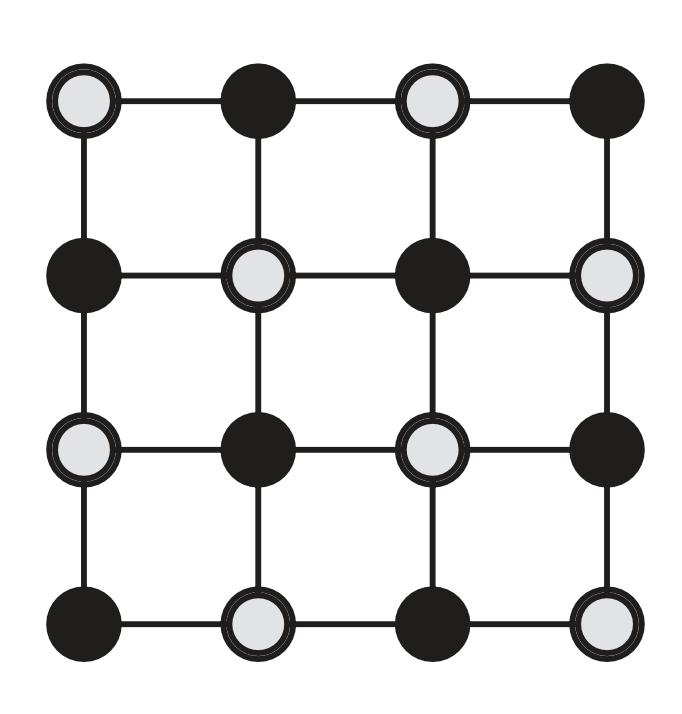
\includegraphics[scale=0.15]{bipartite.png}
    \caption{bipartite}
    \label{}
\end{figure}\end{center}
If the period is $1$ then $\pi$ is the limiting distribution for this chain. If the period is $2$ then $\pi$ can still be interpreted as the limiting expected fraction of time spent in each of the states.


\section{ Countably infinite MC}
Countably infinite MC: Markov Chain in countable infinite state space (e.g. $\mathbb{Z}$). The transition matrix $P$ is infinite large, but the sum of each row converges to $1$.
\subsubsection*{ Chapman Kolmogorov Equations (C-K Equations) also holds: $P(X_{n+m}=j|X_0=i)=(P^{m+n})_{ij}=\sum_{k\in S}(P^{m})_{ik}(P^{n})_{kj}$}
\textbf{Example}:
\begin{enumerate}[(1)]
    \item RW with partially reflecting boundary $S=\{0,1,2,...\}$, $P_{x,x-1}=1-p,P_{x,x+1}=p, P_{0,1}=p, P_{0,0}=1-p$.
    \item Queuing Model: $X_n=$ \# people at time $n$. $S=\{0,1,2,...\}$. $P(x,x-1)=q(1-p)$; $P(x,x+1)=(1-q)p$; $P(x,x)=pq+(1-p)(1-q)$; $P(0,0)=1-p$; $P(0,1)=p$.
\end{enumerate}

\subsubsection*{Difference: For the infinite, irreducible, and aperiodic MC, there may not exist stationary distribution.}
\begin{example}
    For Simple Random Walk: assume there exists a stationary distribution $\pi$, we have
    \begin{equation}
        \begin{aligned}
            \pi_j=\frac{1}{2}(\pi_{j-1}+\pi_{j+1}) \Rightarrow \pi_j-\pi_{j-1}=\pi_{j+1}-\pi_j
        \end{aligned}
        \nonumber
    \end{equation}
    Let the difference between $\pi_j-\pi_{j-1}=\varepsilon$, there doesn't exist solution to
    $$\sum_{i=0}^\infty \pi_i=1; \pi_i=i \varepsilon, i=0,1,...$$
\end{example}

\subsection{Recurrence and Transience}

\subsubsection{Recurrent or Transient State}
Suppose the first return time $T_j=\min\{n>0:X_n=j\}$.

Let the probability of the chain return to $j$ given $X_0=j$ is $$f_j=P(T_j<\infty|X_0=j)$$

\begin{definition}
    A state $j$ is \textbf{recurrent} if $f_j=1$ and \textbf{transient} if $f_j<1$.
\end{definition}

\subsubsection{Recurrent or Transient Class}
(Also class properties: states of a class should be all recurrent or all transient)
\begin{lemma}
    If $i,j$ are in the same class, $i$ is recurrent $\Leftrightarrow$ $j$ is recurrent.
\end{lemma}
\begin{proof}
    Suppose $i$ is recurrent, $P(T_i<\infty|X_0=i)=1$. Since $i\sim j$, $\exists k>0,P_{ij}^k>0$.

    Suppose $P(T_j<\infty|X_0=j)<1$ i.e., $P(T_j=\infty|X_0=j)>0$. Then,
    \begin{equation}
        \begin{aligned}
            P(T_i=\infty|X_0=i)&\geq P(T_i=\infty|X_0=j)P_{ij}^k\\
            &=P(T_i=\infty| T_j=\infty, X_0=j)P(T_j=\infty| X_0=j)P_{ij}^k>0
        \end{aligned}
        \nonumber
    \end{equation}
\end{proof}

\subsubsection{Lemma: Transient Class $\Leftrightarrow$ $\sum_{n=0}^\infty P_{i,i}^n<\infty$}
\begin{lemma}
    An irreducible MC is \textbf{transient} \underline{if and only if} the expected number of visits to a state is finite; i.e. $$\sum_{n=0}^\infty P_{i,i}^n<\infty$$
\end{lemma}
\begin{proof}
    Let the total number of visits $i$ in infinite time is $Y_i=\sum_{n=0}^\infty \mathbf{1}_{X_n=i}$. The expected number is $\mathbb{E}[Y_i|X_0=i]=\sum_{n=0}^\infty P_{i,i}^n$.
    
    $\Leftarrow$: If $i$ is recurrent, the expected total number to visits $i$ in infinite time should be infinite.
    Then, the MC can be proved to be transient if $\mathbb{E}[Y_i|X_0=i]=\sum_{n=0}^\infty P_{i,i}^n<\infty$.

    $\Rightarrow$: Suppose $i$ is transient, let $f_i=P(T_i=\infty|X_0=i)=q>0$ (Probability of not return). Then, the expected number of \underline{returns} to $i$ is (follows geometric distribution)
    \begin{equation}
        \begin{aligned}
            \sum_{n=0}^\infty (1-q)^nqn=q(1-q)\frac{\partial \left(-\sum_{n=0}^\infty(1-q)^n\right)}{\partial q}=q(1-q)\frac{\partial \left(-\frac{1}{q}\right)}{\partial q}=\frac{1-q}{q}
        \end{aligned}
        \nonumber
    \end{equation}
    which also equals to $\mathbb{E}[Y_i|X_0=i]-1 \Rightarrow \mathbb{E}[Y_i|X_0=i]=\frac{1}{q}<\infty$
\end{proof}

\subsubsection{Recurrence/Transience of Simple Random Walk on Lattice}
\textbf{Is the $d$ dimensional SRW recurrent or transient?}

We can first consider $d=1$ case. We want to compute the probability of returning to state $0$ (the same as others). For $2n$ steps trajectories, there are $\begin{pmatrix}
    2n\\
    n
\end{pmatrix}$ trajectories that can return to $0$ and each has probability $\frac{1}{2^{2n}}$.
$$P_{0,0}^{2n}=\begin{pmatrix}
    2n\\
    n
\end{pmatrix}\frac{1}{2^{2n}}=\frac{(2n)!}{n!n!2^{2n}}$$
\textbf{Using Stirling's formula:} $n!\sim\sqrt{2\pi n}\left(\frac{n}{e}\right)^n$ that is $\lim_{n \rightarrow \infty}\frac{n!}{\sqrt{2\pi n}\left(\frac{n}{e}\right)^n}=1$
$$P_{0,0}^{2n}\sim\frac{2\sqrt{\pi n}\left(\frac{2n}{e}\right)^{2n}}{2\pi n\left(\frac{n}{e}\right)^{2n}2^{2n}}=\frac{1}{\sqrt{\pi n}}$$
So the $\sum_{n=N}^\infty P_{0,0}^{2n}=\sum_{n=N}^\infty\frac{1}{\sqrt{\pi}}n^{-\frac{1}{2}}=\infty$.

\textbf{Note:} $n^{-\alpha}$ diverges when $\alpha\in (0,1]$ and converges when $\alpha>1$.

For $d$ dimensions, $$P_{0,0}^{2n}\sim n^{-\frac{d}{2}}$$

\begin{lemma}
    SRW is recurrent when $d=1,2$; SRW is transient when $d\geq 3$.
\end{lemma}



\subsubsection{Null and Positive Recurrence}
$\mu_j= \mathbb{E}[T_j|X_0=j]$
\begin{definition}
    A state $j$ is \textbf{positive recurrent} if it is recurrent and $\mu_j<\infty$. A state $j$ is \textbf{null recurrent} if it is recurrent and $\mu_j=\infty$.
\end{definition}
\textbf{Example of null recurrent:} $P(T_i=n)=\frac{1}{n(n+1)}=\frac{1}{n}-\frac{1}{n+1},n\geq 1$.
\begin{equation}
    \begin{aligned}
        f_i&=\sum_{n=1}^\infty P(T_i=n)=\sum_{n=1}^\infty\left(\frac{1}{n}-\frac{1}{n+1}\right)\Rightarrow \text{ recurrent}\\
        \mu_i&=\sum_{n=1}^\infty nP(T_i=n)=\sum_{n=1}^\infty\frac{1}{n+1}=\infty\Rightarrow \text{ null recurrent}
    \end{aligned}
    \nonumber
\end{equation}

\subsubsection{Stationary Distribution and Limiting Distribution}
Limiting distribution $$\lim_{n \rightarrow \infty}P^{n}_{y,x}=\pi(x),\ \forall x,y\in S$$
Obviously, when a chain is transient, $\lim_{n \rightarrow \infty}P^{n}_{y,x}=0$, there will be no limiting distribution. We can also know $\lim_{n \rightarrow \infty}P^{n}_{y,x}=0$ when the chain is null recurrent.

\begin{lemma}
    For an irreducible MC, $\lim_{n \rightarrow \infty}P^{n}_{y,x}=0$ for each $x,y\in S$ \textbf{if and only if} the chain is transient or null recurrent.
\end{lemma}

\begin{theorem}[Fundamental Theorem for General Discrete Markov Chains]
    An \textbf{irreducible, positive recurrent} MC has a \textbf{unique stationary distribution} $\pi$ (which is positive everywhere) solving the equation
    $$\sum_{y\in S}\pi(y)P(y,x)=\pi(x),\ \forall x\in S$$
    $\pi(j)$ equals to the \textbf{expected visiting time} at $j$ $$\lim_{n \rightarrow \infty}\frac{1}{n}\sum_{k=0}^{n-1}P_{ij}^k=\pi(j)$$
    If in addition, the MC is \textbf{aperiodic}, then $$\lim_{n \rightarrow \infty}P_{ij}^n=\pi(j)$$
    The stationary distribution $\pi$ is also \textbf{inversely} related to the \textbf{expected first return times}. $$\pi(j)=\frac{1}{\mathbb{E}(T_j|X_0=j)}=\frac{1}{\mu_j}$$
    Furthermore, if the irreducible chain is not positive recurrent then there does not exist a stationary distribution.
\end{theorem}

\textbf{Note:} we can prove a MC is not positive recurrent by showing the MC doesn't have a stationary distribution.



\subsection{Differences between Finite and (Countably) Infinite Markov Chains}
\begin{enumerate}
    \item An irreducible MC with finite $S$ has to be recurrent. An irreducible MC with infinite $S$ could be recurrent or transient.
    \item An irreducible MC with finite $S$ has to be positive recurrent. An irreducible recurrent MC with infinite $S$ could be positive recurrent ($\mathbb{E}[T_j|X_0=j]<\infty$) or null recurrent ($\mathbb{E}[T_j|X_0=j]=\infty$).
    \item An irreducible MC with finite $S$ always has a unique stationary distribution. An irreducible recurrent MC with infinite $S$ has a (unique) stationary distribution if and only if the MC is positive recurrent.
\end{enumerate}

\section{Branching Process}
(Sir Francis Galton, 1873) It is a stochastic model for population growth. Let $X_n$ denote the number of individuals at time $n$. At each time interval, each individual will produce a random number of offsprings and then die.

\textit{Two Assumptions:}
\begin{enumerate}[(1)]
    \item Each individual produces offspring with the same probability distribution: there are given non-negative numbers $p_0, p_1, ...$ summing up to $1$ so that the probability of an individual producing $k$ children is $p_k$.
    \item The individuals reproduce independently.
\end{enumerate}

We want to know
\begin{center}
    \textit{"What is the probability that the population eventually becomes extinct?"}
\end{center}

The number of individuals at time $n$, $X_n$ is a MC with state space $S = \{0,1,2,...\} = \mathbb{Z}_+$. Note that $0$ is an absorbing state. Suppose $X_n = k$. Then k individuals produce offspring for the next generation. Let $Y_1,...,Y_k$ be i.i.d random variables with $P(Y_1 = j) = p_j$. Then we can write the transition probabilities as $$P_{k,j}=P(Y_1+\cdots+Y_k=j)$$
Since $P(X_1=0|X_0=i)=p_0^i>0$ for each $i>0$, the \underline{any state $i>0$ must be transient}. From this, it can be shown that, with probability $1$, the chain must either get absorbed in $0$ eventually or approach $\infty$.

\subsection{Extinction Probability in a Branching Process}
\subsubsection{Expectation $\mathbb{E}X_n=\mu^n \mathbb{E}X_0$}
The mean number of offsprings produced by an individual: $$\mu=\sum_{i=0}^\infty i p_i$$
The mean number of individuals in generation $n$,
\begin{equation}
    \begin{aligned}
        \mathbb{E}X_n=\sum_{k=0}^\infty P(X_{n-1}=k)\mathbb{E}(X_n|X_{n-1}=k)=\sum_{k=0}^\infty P(X_{n-1}=k)k\mu=\mu \mathbb{E}X_{n-1}
    \end{aligned}
    \nonumber
\end{equation}
Then, we can get $$\mathbb{E}X_n=\mu^n \mathbb{E}X_0$$

\subsubsection{Lemma: $\mu<1$ $\Rightarrow$ $P(extinction)=1$}
\begin{lemma}
    If $\mu < 1$, then probability of extinction is $1$.
\end{lemma}
\begin{proof}
    We know the event $\{X_{n-1}=0\}\subseteq \{X_{n}=0\}$
    $$P(extinction)=P(\cup_{n=0}^\infty\{X_n=0\})=\lim_{n \rightarrow \infty}P(X_n=0)$$
    \begin{equation}
        \begin{aligned}
            P(X_n\geq 1)=\sum_{k=1}^\infty P(X_n=k)\leq \sum_{k=1}^\infty kP(X_n=k)= \mathbb{E}X_n
        \end{aligned}
        \nonumber
    \end{equation}
    Now, the probability of survival
    \begin{equation}
        \begin{aligned}
            \lim_{n \rightarrow \infty}P(X_n\geq 1)&\leq \lim_{n \rightarrow \infty} \mathbb{E}X_n=\lim_{n \rightarrow \infty} \mu^n \mathbb{E}X_0=0\\
            \Rightarrow \lim_{n \rightarrow \infty}P(X_n\geq 1)&=0
        \end{aligned}
        \nonumber
    \end{equation}
    Then we can conclude $$P(extinction)=\lim_{n \rightarrow \infty}P(X_n=0)=1-\lim_{n \rightarrow \infty}P(X_n\geq 1)=1$$
\end{proof}

If $\mu = 1$, the expected population size remains constant while if $\mu > 1$, the expected population size grows.

\subsubsection{Variance: $Var X_n=\left\{\begin{matrix}
    n\sigma^2,&\mu=1\\
    \sigma^2\mu^{n-1}\frac{\mu^n-1}{\mu-1},&\mu\neq 1
\end{matrix}\right.$}
Let's calculate the variance of $X_n$. We denote the variance of the number of offsprings produced by an individual by $\sigma^2$. By the law of total variance,
\begin{equation}
    \begin{aligned}
        Var X_n&=Var(\mathbb{E} X_n|X_{n-1})+\mathbb{E}Var(X_n|X_{n-1})\\&=Var(\mu X_{n-1})+ \mathbb{E}(\sigma^2 X_{n-1})\\&=\mu^2 Var(X_{n-1})+\sigma^2 \mu^{n-1}\mathbb{E}X_0
    \end{aligned}
    \nonumber
\end{equation}
(Assuming $X_0=1$ with probability $1$)
\begin{equation}
    \begin{aligned}
        Var X_n=\left\{\begin{matrix}
            n\sigma^2,&\mu=1\\
            \sigma^2\mu^{n-1}\frac{\mu^n-1}{\mu-1},&\mu\neq 1
        \end{matrix}\right.
    \end{aligned}
    \nonumber
\end{equation}





To avoid trivial cases, we assume 1.$p_0>0$; 2. $p_0+p_1<1$.

Let $a_n(k)=P(X_n=0|X_0=k)$ and let $a(k)=\lim_{n \rightarrow \infty}a_n(k)$ denote the probability that the population dies out eventually assuming that $X_0=k$.

Since all $k$ individuals act independently, we must have $$a(k)=a(1)^k$$

We simply denote $a(1)$ by $\rho$.
\begin{equation}
    \begin{aligned}
        \rho=a(1)=P(extinction|X_0=1)=\lim_{n \rightarrow \infty}P(X_n=0|X_0=1)
    \end{aligned}
    \nonumber
\end{equation}
By conditioning on the first step, we can write
\begin{equation}
    \begin{aligned}
        \rho=\sum_{k=0}^\infty P(X_1=k|X_0=1)P(extinction|X_1=k)=\sum_{k=0}^\infty p_k\rho^k=\psi(\rho)
    \end{aligned}
    \nonumber
\end{equation}
where $\psi:[0,1] \rightarrow \mathbb{R}$ is given by $\psi(z)=\sum_{k=0}^\infty p_k z^k$. Then the $\rho$ satisfies $z=\psi(z)$

\begin{definition}
    If a random variable $X$ takes values in $\mathbb{Z}$, the \textbf{probability generating function (pgf)} of $X$ is the function $\psi : [0,1] \rightarrow \mathbb{R}$ given by $$\psi(s)=\psi_X(s)=\mathbb{E}(s^X)=\sum_{k=0}^\infty s^k P(X=k)$$
\end{definition}

We now note some important properties of the function $\psi$.
\begin{enumerate}
    \item $\psi'(x)=\sum_{k=1}^\infty x^{k-1}k p_k>0$ for $x\in (0,1)$ $\Rightarrow$ $\psi$ is an \textbf{increasing} function.
    \item $\psi^{''}(x)=\sum_{k=2}^\infty x^{k-2}k(k-1) p_k>0$ for $x\in (0,1)$ $\Rightarrow$ $\psi$ is a \textbf{convex} function.
    \item $\psi(0)=p_0>0$
    \item $\psi(1)=1$
    \item $\psi'(1)=\sum_{k=1}^\infty k p_k=\mu$
    \item \textbf{Probability Generating Functions characterize the distribution}: if two discrete random variables have their pgf the same then they have the same distribution.
    \item $\psi_{X+Y}(s)=\mathbb{E}(s^{X+Y})=\mathbb{E}(s^X)\mathbb{E}(s^Y)=\psi_X(s)\psi_Y(s)$
\end{enumerate}

\begin{center}\begin{figure}[htbp]
    \centering
    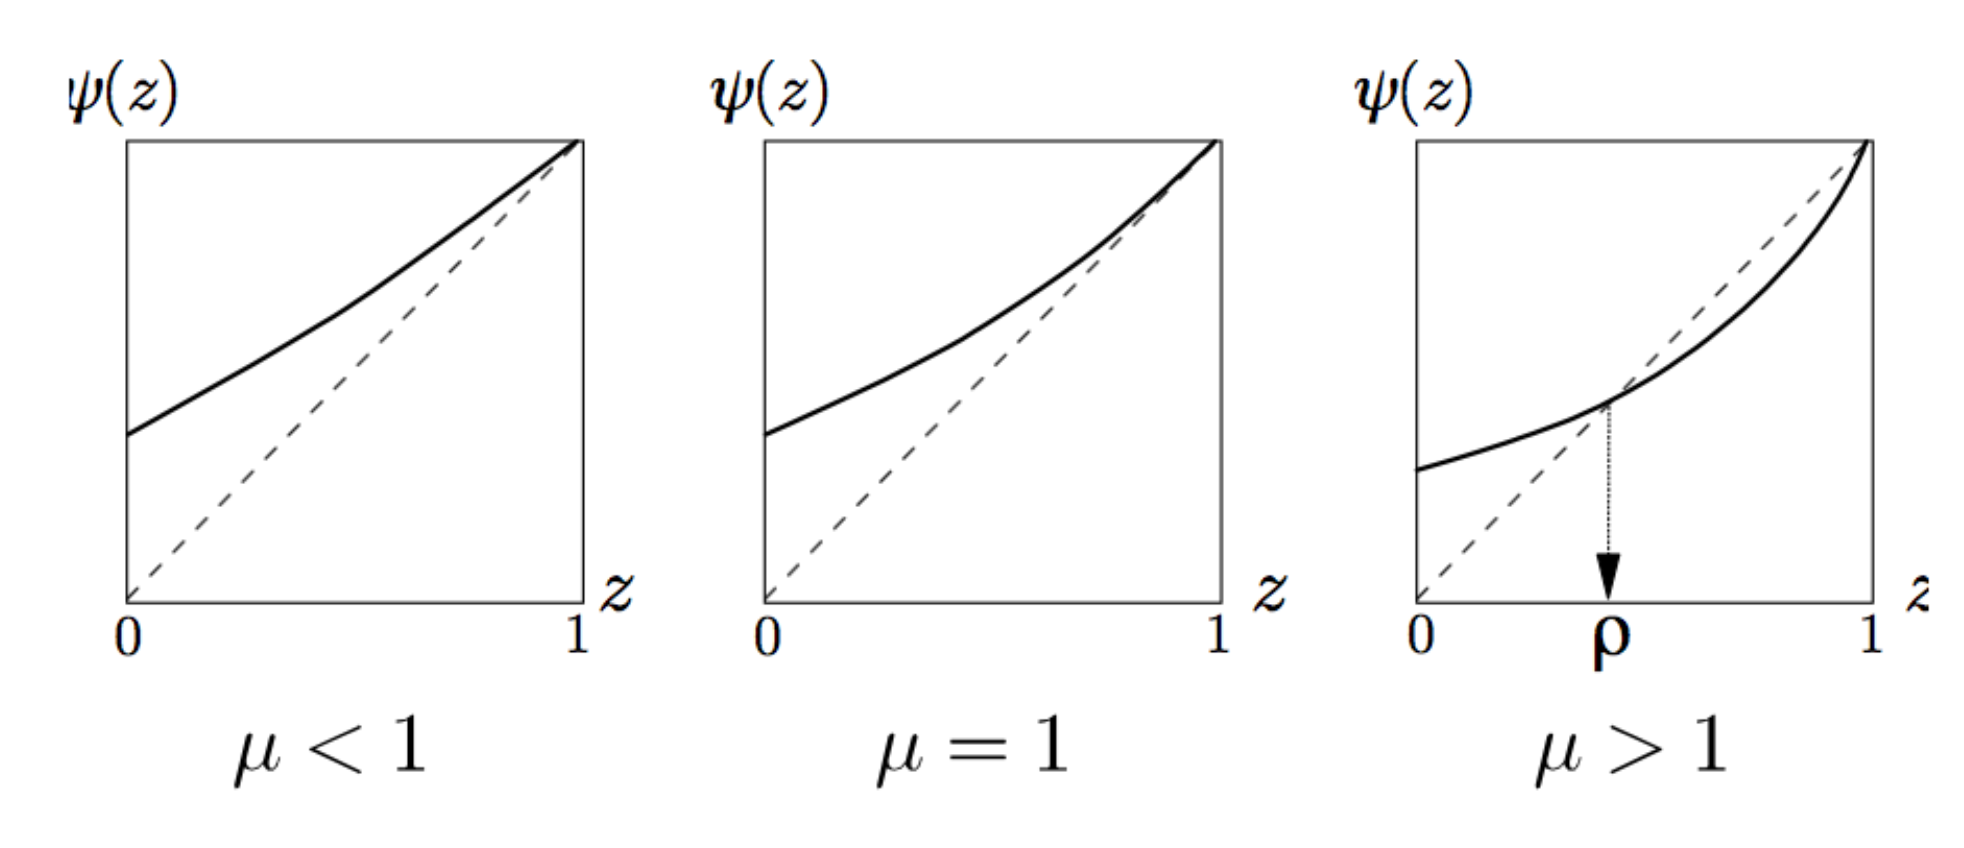
\includegraphics[scale=0.2]{pgf.png}
    \caption{Fixed Point of pgf}
    \label{}
\end{figure}\end{center}





































\end{document}